\subsection{Interprêter la requête et cibler le contenu d'intérêt pour y répondre}

Pour analyser les demandes de l'utilisateur, il faut les traduire en requêtes neurales pour ensuite rechercher dans le texte les passages intéressants. Cela est une étape importante à comprendre avant d'analyser d'avantage ce qui sera expliqué dans les prochaines sections. C'est l'une des choses que peuvent faire les mécanismes d'attention tels qu'introduits par Bahdanau et al. en 2014 \cite{attentionMechanism}. Ces mécanismes sont illustrés à la \autoref{fig:attn}. Son fonctionnement va comme suit. En premier lieu, le texte est lu séquentiellement en entrée (en bas à gauche). Ensuite, une requête est faite pour filtrer ce qui est lu et faire l'alignement d'attention (en bas à droite). Cette requête peut provenir d'un autre réseaux de neurones, mais est ici elle-même générée dans un contexte de traduction automatique. La requête est donc de demander par quoi la phrase devrait débuter lors de ce début de traduction, ce que le décodeur (à droite) peut utiliser pour construire mot par mot une phrase traduite avec une requête à chaque nouveau mot, séquentiellement. Cette requête est à chaque étape comparée à toute l'information à filtrer par le mécanisme d'attention (au centre). C'est ainsi qu'un résultat est formulé par ce calcul du mécanisme d'attention en fonction de la requête demandée (en haut). Les auteurs soutiennent que les mécanismes d'attention sont à explorer plus en profondeur et que cela n'est que leur début. Une certaine exploration de ce mécanisme est faite par Luong et al. en 2015 \cite{attentionBasedApproaches}. Notamment, ils définissent un tel mécanisme comme étant un mini réseaux de neurones dans un plus gros. Ce mini réseaux de neurones sert à déterminer où mettre l'attention, et peut prendre des formes variées, tel qu'un réseaux de neurones linéaire à deux couches, ou bien une comparaison par produit vectoriel de chaque élément à comparer à la requête, en tant que mesure de similarité entre la requête et les éléments d'information où rechercher. \\

\begin{figure*}
  \centering
  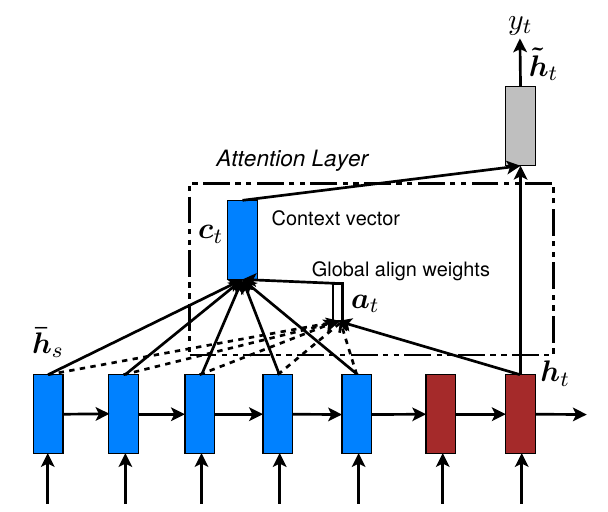
\includegraphics[width=\textwidth, height=0.4\textheight, keepaspectratio]{bahdanauAttentionMechanism2014}
  \caption{Mécanisme d'attention sous sa forme générale, tel qu'introduit par Bahdanau et al. en 2014 \cite{attentionMechanism} et ici raffinés par Luong et al \cite{attentionBasedApproaches} dans cette figure.}
  \label{fig:attn}
\end{figure*}

Il est bien d'avoir les mécanismes d'attention pour faire de la traduction automatique \cite{attentionMechanism}, mais il est tout aussi possible de les utiliser pour trouver dans du texte les passages intéressants en fonction d'une questions. C'est ce que font Cui et al. \cite{squad\string:attentionOverAttention}, tout comme Xiong et al. \cite{squad\string:coattention}, en 2016 sur le jeux de données du SQuAD \cite{squad}, cela suite aux travaux de Google de 2015 lesquels sont détaillés dans la section suivante \cite{readNcomprehend}. Les travaux de Cui et al. sont imagés à la \autoref{fig:coAttn}. La réponse est retournée suite à avoir posé une question dans le texte. Ce réseaux de neurones ressemble à celui de Google, lequel est détaillé à la section suivante.

\begin{figure*}
  \centering
  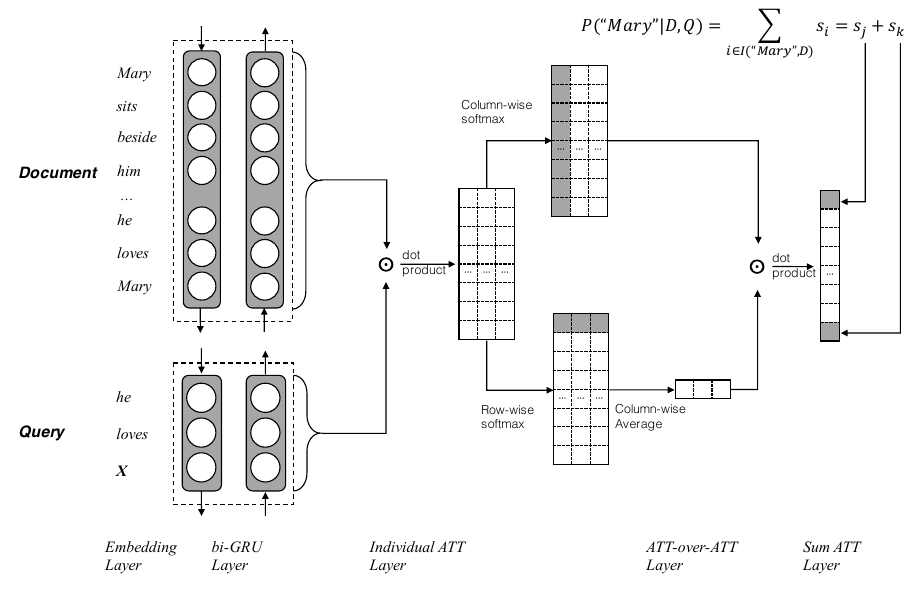
\includegraphics[width=\textwidth, height=0.4\textheight, keepaspectratio]{squadAttentionOverAttention}
  \caption{Réseaux de neurones profond permettant d'analyser un document (en haut à gauche) en fonction d'une requête (en bas à gauche) pour produire une réponse avec l'information trouvée (à droite), par Cui et al. \cite{squad\string:attentionOverAttention}.}
  \label{fig:coAttn}
\end{figure*}
